%%
%% This is file `main.tex',
%% Curated for DocEng 2026
%%
\documentclass[sigconf, review]{acmart}
\usepackage{xcolor}
\usepackage{tikz}
\usepackage{standalone}
\usepackage{makecell}
\usetikzlibrary{shapes.geometric, arrows.meta, positioning, calc, backgrounds}



%%
%% \BibTeX command to typeset BibTeX logo in the docs
\AtBeginDocument{%
  \providecommand\BibTeX{{%
    Bib\TeX}}}

%% Rights management information.
\setcopyright{acmlicensed}
\copyrightyear{2026}
\acmYear{2026}
\acmDOI{XXXXXXX.XXXXXXX}
\acmConference[DocEng '26]{The 26th ACM Symposium on Document Engineering}{August 25--28, 2026}{Fribourg, Switzerland}
\acmISBN{978-1-4503-XXXX-X/26/08}

\begin{document}

\title{Out of Character: Cost-Aware Human-LLM Collaboration for Historical Archives}
\author{Anonymised for review}
%\author{Stergios Konstantinidis}
%\affiliation{%
%  \institution{University of Lausanne}
%  \city{Lausanne}
%  \country{Switzerland}}
%\email{stergios@unil.ch}
%
%\author{Hayman Lotfy}
%\affiliation{%
%  \institution{University of Lausanne}
%  \city{Lausanne}
%  \country{Switzerland}}
%  \email{hayman.lotfy@unil.ch}
%
%\author{Michalis Vlachos}
%\affiliation{%
%  \institution{University of Lausanne}
%  \city{Lausanne}
%  \country{Switzerland}}
%\email{michalis.vlachos@unil.ch}

%\renewcommand{\shortauthors}{Konstantinidis et al.}
\renewcommand{\shortauthors}{Anonymised for review}
\begin{abstract}
OCR transcription errors in historical archives hinder digital search and retrieval. While Large Language Models (LLMs) can correct many of these errors, applying them indiscriminately is costly and may negatively affect already-clean text. We propose a three-tier collaboration framework that routes each text segment to one of: (1) No Correction, (2) LLM Correction, or (3) Human Correction. We introduce a regression-guided routing approach that prioritizes documents by predicted CER improvement, paired with a safeguard layer that detects harmful LLM corrections and routes uncertain documents to human review. With only $<$5\% of the corpus reviewed by human experts, our safeguard achieves 2.55\% CER, a 14\% relative reduction over the All-LLM baseline (2.98\% CER) and substantially outperforming standard confidence-based approaches. By dynamically routing degraded segments to humans and fixable errors to the LLM, the collaborative framework outperforms either corrector in isolation.
\end{abstract}



\begin{CCSXML}
<ccs2012>
 <concept>
  <concept_id>10010405.10010497.10010504.10010505</concept_id>
  <concept_desc>Applied computing~Document analysis</concept_desc>
  <concept_significance>500</concept_significance>
 </concept>
 <concept>
  <concept_id>10010147.10010178.10010179.10010182</concept_id>
  <concept_desc>Computing methodologies~Natural language generation</concept_desc>
  <concept_significance>300</concept_significance>
 </concept>
</ccs2012>
\end{CCSXML}

%\ccsdesc[500]{Applied computing~Document analysis}
%\ccsdesc[300]{Computing methodologies~Natural language generation}

\keywords{OCR Correction, Large Language Models, Historical Newspapers, Cost-Effectiveness, Document Analysis, Human-LLM Collaboration, Binary Routing}



\maketitle

\section{Introduction}
Historical newspaper archives are invaluable for humanities research, yet their OCR transcriptions often suffer from high word-error rates (WER) caused by old typefaces, physical degradation, irregular spelling, and complex layouts~\cite{holley2009good,alex2012digitised,piryani2025evaluating}. Large Language Models (LLMs) can correct many of these errors contextually; however, applying them indiscriminately is costly, unnecessary for clean segments, and risks introducing ``modernization'' errors that alter historical spelling conventions.

To address these issues, we propose a three-tier collaboration framework that routes each raw OCR segment to one of: (1) No Correction, retaining the OCR text; (2) LLM Correction, applying automated post-editing; or (3) Human Correction, delegating highly degraded text for expert review. We evaluate our routing strategies on a historical Swiss newspaper corpus (1733--1945), predicting optimal delegation paths from raw OCR features alone.

Our main \textbf{contributions} are:
\begin{itemize}
    \item A cost-aware routing framework coordinating OCR outputs, LLMs, and human reviewers, with a regression-guided routing strategy.
    \item A regression-guided routing approach with a safeguard layer that detects harmful LLM corrections and routes uncertain documents to human review under a small budget constraint ($<$5\% of the corpus).
    \item An evaluation on a historical Swiss newspaper corpus (1733--1945) showing our safeguard achieves 2.55\% CER with only $<$5\% of the corpus reviewed by human experts, a 14\% relative reduction over the All-LLM baseline (2.98\% CER) and substantially outperforming confidence-based approaches.
\end{itemize}


\section{Related Work}
Post-OCR correction is transitioning from rule-based and statistical methods, such as noisy-channel models \cite{kissos_ocr_2016}, to deep learning and Large Language Models~\cite{nguyen2021survey}. Recent studies show that LLMs can improve historical newspaper transcriptions \cite{thomas2024leveraging}, though performance remains sensitive to prompt design, language, and script complexity \cite{boros2024post, sohail2024decipheringunderservedbenchmarkingllm}. While traditional dictionary-based spell-checkers struggle with real-word errors (which account for up to 59.0\% of OCR noise \cite{10.1007/978-3-031-70442-0_13}), they can also trigger modernization traps by changing valid archaic spellings (e.g., historical French \textit{seroit} to modern \textit{serait}) \cite{hammarstrom2025investigation}.

\medskip\noindent\textbf{Confidence-Aware Detection and Hybrid Models.}
OCR engine confidence scores are frequently used to locate errors. Hemmer et al. \cite{10.1007/978-3-031-70442-0_13} propose ConfBERT, which fuses token confidence scores with language representations for binary error detection. Unlike token-level error detection, our framework operates at the document-segment level to make three-class routing decisions based on surface, spelling, and metadata features.

\medskip\noindent\textbf{Cost-Aware Routing.}
As LLM adoption grows, cost-aware routers like RouteLLM \cite{Ong2025RouteLLMLT, li2025costaware} learn to route queries between strong and weak models. Similarly, bandit-based frameworks choose among multiple LLMs \cite{panda2025pilot, wang2025barp}. Complementary to this, our work addresses the binary decision of whether to invoke LLM correction at all, using lightweight, domain-specific features rather than learned embeddings.




\section{Methodology}

We frame OCR post-correction as a three-tier \emph{human-LLM collaboration} framework: rather than correcting every segment using either the LLM or a human reviewer, we choose the most cost-effective path for each segment using only features available from the raw OCR output (see Fig \ref{fig:methodology}). This section details our collaboration tiers, the cost model, the threshold parameter, and the learned routing classifiers.

\begin{figure}[ht]
\centering
\resizebox{\linewidth}{!}{% overview_tikz.tex  –  Three-tier Human-LLM Collaboration Overview
% Include in paper:  \resizebox{\linewidth}{!}{% overview_tikz.tex  –  Three-tier Human-LLM Collaboration Overview
% Include in paper:  \resizebox{\linewidth}{!}{% overview_tikz.tex  –  Three-tier Human-LLM Collaboration Overview
% Include in paper:  \resizebox{\linewidth}{!}{\input{paper/figures/overview_tikz.tex}}
%
% LAYOUT – uniform 1.2 cm gap between node edges:
%   Doc stack A :  x 0.00 – 1.85   (centre 0.93)
%   gap 1.2
%   ML Model  B :  x 3.05 – 5.85   (centre 4.45,  width 2.8)
%   gap 1.2
%   Tier boxes D:  x 7.05 – 9.65   (centre 8.35,  width 2.6)
%   gap 1.2
%   Doc stack E :  x 10.85 – 12.70  (centre 11.63)
%
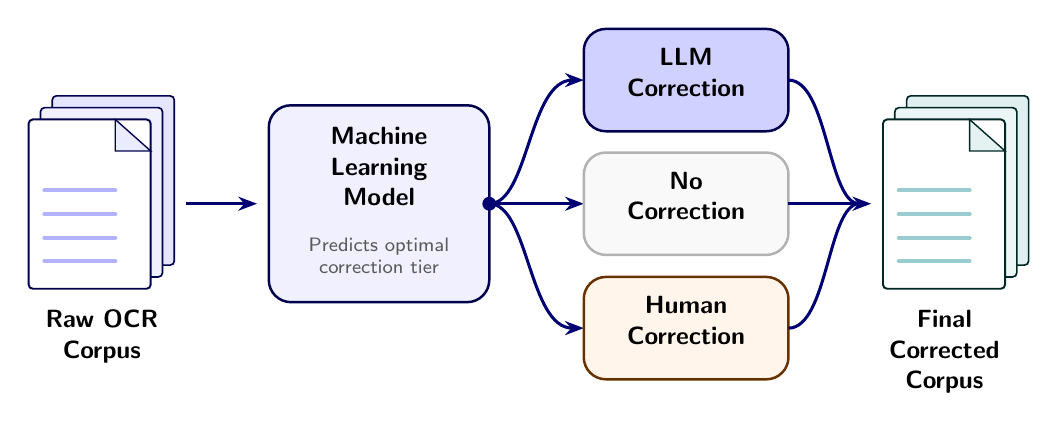
\begin{tikzpicture}[
    % ── colour palette ──
    blueMain/.style  = {draw=blue!30!black, fill=blue!6,
                        rounded corners=8pt, line width=0.9pt},
    blueAccent/.style= {draw=blue!30!black, fill=blue!18!white,
                        rounded corners=8pt, line width=0.9pt},
    orangeBox/.style = {draw=orange!40!black, fill=orange!8!white,
                        rounded corners=8pt, line width=0.9pt},
    keepBox/.style   = {draw=gray!60, fill=gray!5,
                        rounded corners=8pt, line width=0.9pt},
    % ── arrows ──
    arr/.style       = {-{Stealth[scale=0.85]}, line width=1.1pt,
                        blue!45!black},
    % ── text styles ──
    mainLabel/.style = {font=\sffamily\bfseries\small, align=center},
    subLabel/.style  = {font=\sffamily\scriptsize, align=center,
                        text=gray!70!black},
]

\def\midY{1.08}  % vertical centreline

% =====================================================================
% Stage A   RAW OCR CORPUS   (x = 0 – 1.85)
% =====================================================================
\begin{scope}[shift={(0,0)}]
  \draw[blue!30!black, fill=blue!10, rounded corners=1.5pt, line width=0.6pt]
    (0.3,0.3) -- (0.3,2.45) -- (1.85,2.45) -- (1.85,0.3) -- cycle;
  \draw[blue!30!black, fill=blue!6, rounded corners=1.5pt, line width=0.6pt]
    (0.15,0.15) -- (0.15,2.3) -- (1.7,2.3) -- (1.7,0.15) -- cycle;
  \draw[blue!30!black, fill=white, rounded corners=1.5pt, line width=0.7pt]
    (0,0) -- (0,2.15) -- (1.55,2.15) -- (1.55,0) -- cycle;
  \draw[blue!30!black, fill=blue!8, line width=0.5pt]
    (1.1,2.15) -- (1.1,1.75) -- (1.55,1.75) -- cycle;
  \foreach \y in {0.35,0.65,0.95,1.25}{
    \draw[blue!30, line width=1.5pt, line cap=round]
      (0.2,\y) -- ++(0.9,0);
  }
\end{scope}
\node[mainLabel, below] at (0.93,-0.15) {Raw OCR\\Corpus};

% =====================================================================
% Arrow A → B   (gap 1.2:  1.85 → 3.05)
% =====================================================================
\draw[arr] (2.0,\midY) -- (2.9,\midY);

% =====================================================================
% Stage B   MACHINE LEARNING MODEL   (x = 3.05 – 5.85, centre 4.45)
% =====================================================================
\node[blueMain, minimum width=2.8cm, minimum height=2.5cm] (mlbox)
  at (4.45,\midY) {};
\node[mainLabel] at (4.45,1.55) {Machine\\Learning\\Model};
\node[subLabel]  at (4.45,0.42) {Predicts optimal\\correction tier};

% =====================================================================
% Branching junction (at ML box right edge = 5.85)
% =====================================================================
\fill[blue!45!black] (5.85,\midY) circle (2.5pt);

% upper branch  →  LLM Correction
\draw[arr] (5.85,\midY) .. controls (6.35,\midY) and (6.35,2.65)
           .. (7.05,2.65);
% middle branch  →  No Correction
\draw[arr] (5.85,\midY) -- (7.05,\midY);
% lower branch  →  Human Correction
\draw[arr] (5.85,\midY) .. controls (6.35,\midY) and (6.35,-0.5)
           .. (7.05,-0.5);

% =====================================================================
% Stage D   TIER BOXES   (x = 7.05 – 9.65, centre 8.35)
% =====================================================================
% LLM Correction
\node[blueAccent, minimum width=2.6cm, minimum height=1.3cm] (llm)
  at (8.35, 2.65) {};
\node[mainLabel] at (8.35, 2.75) {LLM\\Correction};

% No Correction
\node[keepBox, minimum width=2.6cm, minimum height=1.3cm] (keep)
  at (8.35, \midY) {};
\node[mainLabel] at (8.35, 1.18) {No\\Correction};

% Human Correction
\node[orangeBox, minimum width=2.6cm, minimum height=1.3cm] (human)
  at (8.35, -0.5) {};
\node[mainLabel] at (8.35, -0.4) {Human\\Correction};

% =====================================================================
% Merge D → E   (gap 1.2:  9.65 → 10.85)
% =====================================================================
\draw[blue!45!black, line width=1.1pt]
  (9.65,2.65) .. controls (10.15,2.65) and (10.15,\midY)
  .. (10.55,\midY);
\draw[blue!45!black, line width=1.1pt]
  (9.65,\midY) -- (10.55,\midY);
\draw[blue!45!black, line width=1.1pt]
  (9.65,-0.5) .. controls (10.15,-0.5) and (10.15,\midY)
  .. (10.55,\midY);
% final arrow
\draw[arr] (10.55,\midY) -- (10.7,\midY);

% =====================================================================
% Stage E   FINAL CORRECTED CORPUS   (x = 10.85 – 12.70)
% =====================================================================
\begin{scope}[shift={(10.85,0)}]
  \draw[teal!30!black, fill=teal!12, rounded corners=1.5pt, line width=0.6pt]
    (0.3,0.3) -- (0.3,2.45) -- (1.85,2.45) -- (1.85,0.3) -- cycle;
  \draw[teal!30!black, fill=teal!7, rounded corners=1.5pt, line width=0.6pt]
    (0.15,0.15) -- (0.15,2.3) -- (1.7,2.3) -- (1.7,0.15) -- cycle;
  \draw[teal!30!black, fill=white, rounded corners=1.5pt, line width=0.7pt]
    (0,0) -- (0,2.15) -- (1.55,2.15) -- (1.55,0) -- cycle;
  \draw[teal!30!black, fill=teal!10, line width=0.5pt]
    (1.1,2.15) -- (1.1,1.75) -- (1.55,1.75) -- cycle;
  \foreach \y in {0.35,0.65,0.95,1.25}{
    \draw[teal!40, line width=1.5pt, line cap=round]
      (0.2,\y) -- ++(0.9,0);
  }
\end{scope}
\node[mainLabel, below] at (11.63,-0.15) {Final\\Corrected\\Corpus};

\end{tikzpicture}}
%
% LAYOUT – uniform 1.2 cm gap between node edges:
%   Doc stack A :  x 0.00 – 1.85   (centre 0.93)
%   gap 1.2
%   ML Model  B :  x 3.05 – 5.85   (centre 4.45,  width 2.8)
%   gap 1.2
%   Tier boxes D:  x 7.05 – 9.65   (centre 8.35,  width 2.6)
%   gap 1.2
%   Doc stack E :  x 10.85 – 12.70  (centre 11.63)
%
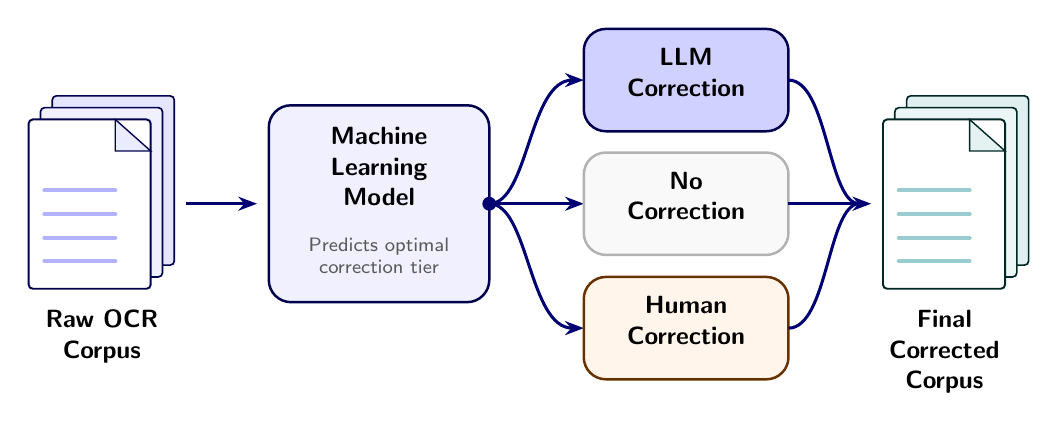
\begin{tikzpicture}[
    % ── colour palette ──
    blueMain/.style  = {draw=blue!30!black, fill=blue!6,
                        rounded corners=8pt, line width=0.9pt},
    blueAccent/.style= {draw=blue!30!black, fill=blue!18!white,
                        rounded corners=8pt, line width=0.9pt},
    orangeBox/.style = {draw=orange!40!black, fill=orange!8!white,
                        rounded corners=8pt, line width=0.9pt},
    keepBox/.style   = {draw=gray!60, fill=gray!5,
                        rounded corners=8pt, line width=0.9pt},
    % ── arrows ──
    arr/.style       = {-{Stealth[scale=0.85]}, line width=1.1pt,
                        blue!45!black},
    % ── text styles ──
    mainLabel/.style = {font=\sffamily\bfseries\small, align=center},
    subLabel/.style  = {font=\sffamily\scriptsize, align=center,
                        text=gray!70!black},
]

\def\midY{1.08}  % vertical centreline

% =====================================================================
% Stage A   RAW OCR CORPUS   (x = 0 – 1.85)
% =====================================================================
\begin{scope}[shift={(0,0)}]
  \draw[blue!30!black, fill=blue!10, rounded corners=1.5pt, line width=0.6pt]
    (0.3,0.3) -- (0.3,2.45) -- (1.85,2.45) -- (1.85,0.3) -- cycle;
  \draw[blue!30!black, fill=blue!6, rounded corners=1.5pt, line width=0.6pt]
    (0.15,0.15) -- (0.15,2.3) -- (1.7,2.3) -- (1.7,0.15) -- cycle;
  \draw[blue!30!black, fill=white, rounded corners=1.5pt, line width=0.7pt]
    (0,0) -- (0,2.15) -- (1.55,2.15) -- (1.55,0) -- cycle;
  \draw[blue!30!black, fill=blue!8, line width=0.5pt]
    (1.1,2.15) -- (1.1,1.75) -- (1.55,1.75) -- cycle;
  \foreach \y in {0.35,0.65,0.95,1.25}{
    \draw[blue!30, line width=1.5pt, line cap=round]
      (0.2,\y) -- ++(0.9,0);
  }
\end{scope}
\node[mainLabel, below] at (0.93,-0.15) {Raw OCR\\Corpus};

% =====================================================================
% Arrow A → B   (gap 1.2:  1.85 → 3.05)
% =====================================================================
\draw[arr] (2.0,\midY) -- (2.9,\midY);

% =====================================================================
% Stage B   MACHINE LEARNING MODEL   (x = 3.05 – 5.85, centre 4.45)
% =====================================================================
\node[blueMain, minimum width=2.8cm, minimum height=2.5cm] (mlbox)
  at (4.45,\midY) {};
\node[mainLabel] at (4.45,1.55) {Machine\\Learning\\Model};
\node[subLabel]  at (4.45,0.42) {Predicts optimal\\correction tier};

% =====================================================================
% Branching junction (at ML box right edge = 5.85)
% =====================================================================
\fill[blue!45!black] (5.85,\midY) circle (2.5pt);

% upper branch  →  LLM Correction
\draw[arr] (5.85,\midY) .. controls (6.35,\midY) and (6.35,2.65)
           .. (7.05,2.65);
% middle branch  →  No Correction
\draw[arr] (5.85,\midY) -- (7.05,\midY);
% lower branch  →  Human Correction
\draw[arr] (5.85,\midY) .. controls (6.35,\midY) and (6.35,-0.5)
           .. (7.05,-0.5);

% =====================================================================
% Stage D   TIER BOXES   (x = 7.05 – 9.65, centre 8.35)
% =====================================================================
% LLM Correction
\node[blueAccent, minimum width=2.6cm, minimum height=1.3cm] (llm)
  at (8.35, 2.65) {};
\node[mainLabel] at (8.35, 2.75) {LLM\\Correction};

% No Correction
\node[keepBox, minimum width=2.6cm, minimum height=1.3cm] (keep)
  at (8.35, \midY) {};
\node[mainLabel] at (8.35, 1.18) {No\\Correction};

% Human Correction
\node[orangeBox, minimum width=2.6cm, minimum height=1.3cm] (human)
  at (8.35, -0.5) {};
\node[mainLabel] at (8.35, -0.4) {Human\\Correction};

% =====================================================================
% Merge D → E   (gap 1.2:  9.65 → 10.85)
% =====================================================================
\draw[blue!45!black, line width=1.1pt]
  (9.65,2.65) .. controls (10.15,2.65) and (10.15,\midY)
  .. (10.55,\midY);
\draw[blue!45!black, line width=1.1pt]
  (9.65,\midY) -- (10.55,\midY);
\draw[blue!45!black, line width=1.1pt]
  (9.65,-0.5) .. controls (10.15,-0.5) and (10.15,\midY)
  .. (10.55,\midY);
% final arrow
\draw[arr] (10.55,\midY) -- (10.7,\midY);

% =====================================================================
% Stage E   FINAL CORRECTED CORPUS   (x = 10.85 – 12.70)
% =====================================================================
\begin{scope}[shift={(10.85,0)}]
  \draw[teal!30!black, fill=teal!12, rounded corners=1.5pt, line width=0.6pt]
    (0.3,0.3) -- (0.3,2.45) -- (1.85,2.45) -- (1.85,0.3) -- cycle;
  \draw[teal!30!black, fill=teal!7, rounded corners=1.5pt, line width=0.6pt]
    (0.15,0.15) -- (0.15,2.3) -- (1.7,2.3) -- (1.7,0.15) -- cycle;
  \draw[teal!30!black, fill=white, rounded corners=1.5pt, line width=0.7pt]
    (0,0) -- (0,2.15) -- (1.55,2.15) -- (1.55,0) -- cycle;
  \draw[teal!30!black, fill=teal!10, line width=0.5pt]
    (1.1,2.15) -- (1.1,1.75) -- (1.55,1.75) -- cycle;
  \foreach \y in {0.35,0.65,0.95,1.25}{
    \draw[teal!40, line width=1.5pt, line cap=round]
      (0.2,\y) -- ++(0.9,0);
  }
\end{scope}
\node[mainLabel, below] at (11.63,-0.15) {Final\\Corrected\\Corpus};

\end{tikzpicture}}
%
% LAYOUT – uniform 1.2 cm gap between node edges:
%   Doc stack A :  x 0.00 – 1.85   (centre 0.93)
%   gap 1.2
%   ML Model  B :  x 3.05 – 5.85   (centre 4.45,  width 2.8)
%   gap 1.2
%   Tier boxes D:  x 7.05 – 9.65   (centre 8.35,  width 2.6)
%   gap 1.2
%   Doc stack E :  x 10.85 – 12.70  (centre 11.63)
%
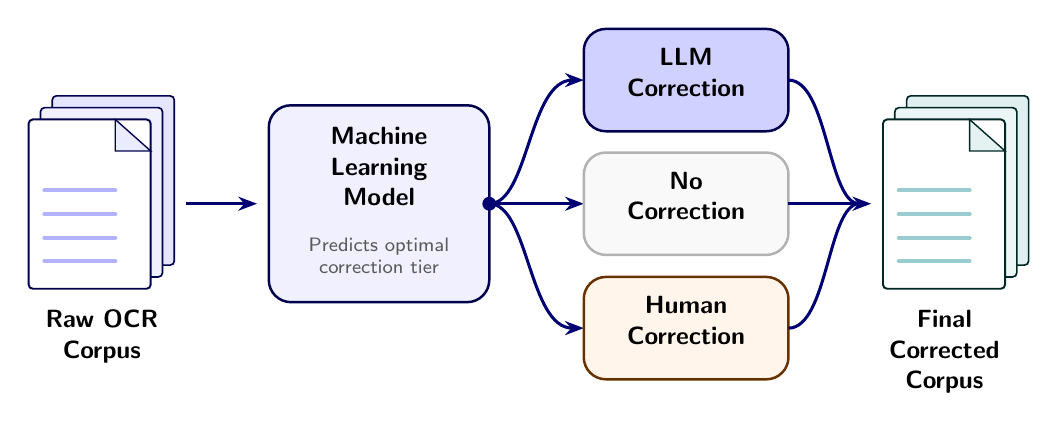
\begin{tikzpicture}[
    % ── colour palette ──
    blueMain/.style  = {draw=blue!30!black, fill=blue!6,
                        rounded corners=8pt, line width=0.9pt},
    blueAccent/.style= {draw=blue!30!black, fill=blue!18!white,
                        rounded corners=8pt, line width=0.9pt},
    orangeBox/.style = {draw=orange!40!black, fill=orange!8!white,
                        rounded corners=8pt, line width=0.9pt},
    keepBox/.style   = {draw=gray!60, fill=gray!5,
                        rounded corners=8pt, line width=0.9pt},
    % ── arrows ──
    arr/.style       = {-{Stealth[scale=0.85]}, line width=1.1pt,
                        blue!45!black},
    % ── text styles ──
    mainLabel/.style = {font=\sffamily\bfseries\small, align=center},
    subLabel/.style  = {font=\sffamily\scriptsize, align=center,
                        text=gray!70!black},
]

\def\midY{1.08}  % vertical centreline

% =====================================================================
% Stage A   RAW OCR CORPUS   (x = 0 – 1.85)
% =====================================================================
\begin{scope}[shift={(0,0)}]
  \draw[blue!30!black, fill=blue!10, rounded corners=1.5pt, line width=0.6pt]
    (0.3,0.3) -- (0.3,2.45) -- (1.85,2.45) -- (1.85,0.3) -- cycle;
  \draw[blue!30!black, fill=blue!6, rounded corners=1.5pt, line width=0.6pt]
    (0.15,0.15) -- (0.15,2.3) -- (1.7,2.3) -- (1.7,0.15) -- cycle;
  \draw[blue!30!black, fill=white, rounded corners=1.5pt, line width=0.7pt]
    (0,0) -- (0,2.15) -- (1.55,2.15) -- (1.55,0) -- cycle;
  \draw[blue!30!black, fill=blue!8, line width=0.5pt]
    (1.1,2.15) -- (1.1,1.75) -- (1.55,1.75) -- cycle;
  \foreach \y in {0.35,0.65,0.95,1.25}{
    \draw[blue!30, line width=1.5pt, line cap=round]
      (0.2,\y) -- ++(0.9,0);
  }
\end{scope}
\node[mainLabel, below] at (0.93,-0.15) {Raw OCR\\Corpus};

% =====================================================================
% Arrow A → B   (gap 1.2:  1.85 → 3.05)
% =====================================================================
\draw[arr] (2.0,\midY) -- (2.9,\midY);

% =====================================================================
% Stage B   MACHINE LEARNING MODEL   (x = 3.05 – 5.85, centre 4.45)
% =====================================================================
\node[blueMain, minimum width=2.8cm, minimum height=2.5cm] (mlbox)
  at (4.45,\midY) {};
\node[mainLabel] at (4.45,1.55) {Machine\\Learning\\Model};
\node[subLabel]  at (4.45,0.42) {Predicts optimal\\correction tier};

% =====================================================================
% Branching junction (at ML box right edge = 5.85)
% =====================================================================
\fill[blue!45!black] (5.85,\midY) circle (2.5pt);

% upper branch  →  LLM Correction
\draw[arr] (5.85,\midY) .. controls (6.35,\midY) and (6.35,2.65)
           .. (7.05,2.65);
% middle branch  →  No Correction
\draw[arr] (5.85,\midY) -- (7.05,\midY);
% lower branch  →  Human Correction
\draw[arr] (5.85,\midY) .. controls (6.35,\midY) and (6.35,-0.5)
           .. (7.05,-0.5);

% =====================================================================
% Stage D   TIER BOXES   (x = 7.05 – 9.65, centre 8.35)
% =====================================================================
% LLM Correction
\node[blueAccent, minimum width=2.6cm, minimum height=1.3cm] (llm)
  at (8.35, 2.65) {};
\node[mainLabel] at (8.35, 2.75) {LLM\\Correction};

% No Correction
\node[keepBox, minimum width=2.6cm, minimum height=1.3cm] (keep)
  at (8.35, \midY) {};
\node[mainLabel] at (8.35, 1.18) {No\\Correction};

% Human Correction
\node[orangeBox, minimum width=2.6cm, minimum height=1.3cm] (human)
  at (8.35, -0.5) {};
\node[mainLabel] at (8.35, -0.4) {Human\\Correction};

% =====================================================================
% Merge D → E   (gap 1.2:  9.65 → 10.85)
% =====================================================================
\draw[blue!45!black, line width=1.1pt]
  (9.65,2.65) .. controls (10.15,2.65) and (10.15,\midY)
  .. (10.55,\midY);
\draw[blue!45!black, line width=1.1pt]
  (9.65,\midY) -- (10.55,\midY);
\draw[blue!45!black, line width=1.1pt]
  (9.65,-0.5) .. controls (10.15,-0.5) and (10.15,\midY)
  .. (10.55,\midY);
% final arrow
\draw[arr] (10.55,\midY) -- (10.7,\midY);

% =====================================================================
% Stage E   FINAL CORRECTED CORPUS   (x = 10.85 – 12.70)
% =====================================================================
\begin{scope}[shift={(10.85,0)}]
  \draw[teal!30!black, fill=teal!12, rounded corners=1.5pt, line width=0.6pt]
    (0.3,0.3) -- (0.3,2.45) -- (1.85,2.45) -- (1.85,0.3) -- cycle;
  \draw[teal!30!black, fill=teal!7, rounded corners=1.5pt, line width=0.6pt]
    (0.15,0.15) -- (0.15,2.3) -- (1.7,2.3) -- (1.7,0.15) -- cycle;
  \draw[teal!30!black, fill=white, rounded corners=1.5pt, line width=0.7pt]
    (0,0) -- (0,2.15) -- (1.55,2.15) -- (1.55,0) -- cycle;
  \draw[teal!30!black, fill=teal!10, line width=0.5pt]
    (1.1,2.15) -- (1.1,1.75) -- (1.55,1.75) -- cycle;
  \foreach \y in {0.35,0.65,0.95,1.25}{
    \draw[teal!40, line width=1.5pt, line cap=round]
      (0.2,\y) -- ++(0.9,0);
  }
\end{scope}
\node[mainLabel, below] at (11.63,-0.15) {Final\\Corrected\\Corpus};

\end{tikzpicture}}
\caption{Overview of our three-tier, cost-aware human-LLM collaboration framework.}
\label{fig:methodology}
\vspace{-1.5em}
\end{figure}

\medskip\noindent\textbf{Three-Tier Collaboration Model.}
Let $\mathcal{D} = \{d_1, \dots, d_n\}$ be a corpus of segments. Each segment $d_i$ has a raw OCR transcription $d_i^{\text{raw}}$, a potential LLM-corrected version $d_i^{\text{corr}}$, and a ground-truth human-corrected version $d_i^{\text{human}}$ (assumed to have zero errors). 
To handle severely degraded content, we explicitly include OCR failures where the engine produced no output, setting $d_i^{\text{raw}} = \text{``''}$ with a default raw $WER(d_i^{\text{raw}}) = 1.0$.
We define three correction paths based on the raw and corrected error rates:
\begin{itemize}
    \item \textbf{No Correction (Class 0):} Bypassed if $WER(d_i^{\text{raw}}) = 0$ to avoid API cost and prevent modernization errors.
    \item \textbf{LLM Correction (Class 1):} Accepted if $WER(d_i^{\text{raw}}) > 0$ and the LLM brings the residual error under a quality threshold $x$ ($WER(d_i^{\text{corr}}) \leq x$).
    \item \textbf{Human Correction (Class 2):} Routed to human review if $WER(d_i^{\text{raw}}) > 0$ and the LLM's corrected version remains poor ($WER(d_i^{\text{corr}}) > x$).
\end{itemize}

\medskip\noindent\textbf{Cost Model.}
Segments represent newspaper blocks averaging ~220 characters (~35 words). Class 0 carries zero cost. Class 1 (LLM) carries an API cost. Class 2 (Human) carries a time cost of $T_{\text{human}} = 4$ minutes per segment (15 segments/hour) to compare the OCR with the historical page image. For an hourly wage $W$, the human segment cost is $C_{\text{human}} = W / 15$ (e.g., \$1.00 at \$15/hour wage, \$2.00 at \$30/hour wage). Under current pricing, the LLM correction cost is three orders of magnitude smaller than the human cost, making the routing decision almost entirely a question of human workload minimization.

\medskip\noindent\textbf{OCR, LLMs, and Prompt Design.}
To evaluate correction generalizability, we run three OCR engines: PaddleOCR~v3~\cite{cui2025paddleocr}, EasyOCR\footnote{\url{https://github.com/JaidedAI/EasyOCR}}, and Tesseract~v5~\cite{tesseractOCR}. Post-correction is performed using six LLMs, spanning closed-source (Gemini~3 Flash, GPT-4o, Claude~3.5 Haiku)\cite{google2025gemini3flash,openai2024gpt4osystemcard, anthropic2024claude35haiku} and open-weight (Qwen~2.5-72B, Llama~3.3-70B, Gemma~4~31B) \cite{qwen2024qwen25,meta2024llama33,google2026gemma4} models. For each model, we evaluate ten distinct prompt templates of increasing complexity: (i)~\emph{Basic} (Prompts 1--2) provide direct, zero-shot instructions focused on raw text recovery, spacing, and punctuation; (ii)~\emph{Intermediate} (Prompts 3--6) introduce historical rules to preserve archaic French orthography and resolve standard typographic confusions (e.g., long `s'~\textit{f}/\textit{s} confusion); (iii)~\emph{Expert/Master} (Prompts 7--10) integrate in-context few-shot exemplars, structured Chain-of-Thought reasoning steps, and strict output formatting constraints to eliminate conversational preambles. Due to space limits, we report results using Tesseract and Gemini~3 Flash, which represent the optimal quality-cost configuration; results for other models and the full prompt ablation study are available in our code repository.



\medskip\noindent\textbf{Regression-Guided Routing with Safeguard.}
Rather than casting routing as classification, we adopt a two-step approach:

\smallskip\noindent\emph{Step 1: Priority ordering.}
A LassoCV regression model predicts the continuous improvement in CER ($\Delta\text{CER} = \text{CER}_{\text{raw}} - \text{CER}_{\text{corr}}$) from the raw-OCR feature vector $\phi(d_i)$. A positive $\Delta\text{CER}$ indicates that LLM correction reduces error. Documents are sorted by predicted $\Delta\text{CER}$ (most beneficial first) and corrected incrementally.

\smallskip\noindent\emph{Step 2: Per-document safeguard.}
As each document is processed in the priority order, a safeguard classifier decides its correction path. We train a logistic regression model under 10-fold CV to estimate $P(\Delta\text{CER} \geq 0 \mid \phi(d_i))$---the probability that LLM correction is safe (i.e., does not increase error). For each document:
\begin{itemize}
    \item If $P \geq 0.5$: the LLM correction is \textbf{accepted} (correction is likely safe).
    \item If $P < 0.5$ and the human budget $B$ is not exhausted: the document is \textbf{routed to human review} (perfect correction, CER $= 0$).
    \item If $P < 0.5$ and the budget is exhausted: the document \textbf{falls back to LLM correction}.
\end{itemize}
We set $B <5 \%$ of the corpus. This design ensures that the safeguard can only improve upon the unguarded routing curve, since it replaces a subset of potentially harmful LLM corrections with perfect human corrections. All models are evaluated under Leave-One-Out CV on the 597 scanned segments.

\section{Experimental Results}
\label{sec:experiments}

We structure the evaluation around two research questions:
\begin{itemize}
    \item \textbf{RQ1:} How effectively does regression-guided routing prioritize LLM corrections, and can a safeguard with a small human budget improve quality?
    \item \textbf{RQ2:} Can post-LLM safeguard classifiers detect and intercept harmful corrections under a fixed operational budget?
\end{itemize}
All code, data, prompts, and per-model results are available in an anonymized
repository.\footnote{\url{https://anonymous.4open.science/r/DocEng_public-8FC9/}}


\medskip\noindent\textbf{Corpus and annotation.}
We use the corpus summarized in Table~\ref{tab:corpus}: 609 text segments from nine Swiss historical newspapers (1733--1945) in the digital archives of the Canton of Vaud. Three French-speaking annotators produced fidelity-oriented
transcriptions that preserve historical spelling and source anomalies. We report
WER and CER, computed after a topological normalization step that unifies
historical character variants and spacing.



\begin{table}[h]
\centering
\caption{Corpus composition by newspaper publication.}
\vspace{-\baselineskip}
\label{tab:corpus}
\resizebox{0.8\columnwidth}{!}{%
\begin{tabular}{@{}lcccc@{}}
\toprule
\textbf{Newspaper} & \textbf{Dates} & \textbf{Issues} & \textbf{Pages} & \textbf{Text} \\
 & & & & \textbf{segments} \\ \midrule
La Revue                       & 1875--1945 & 4 & 5  & 139 \\
Feuille d'Avis & 1762--1841 & 4 & 13 & 131 \\
Tribune de Lausanne                        & 1912       & 3 & 4  & 105 \\
Nouvelliste Vaudois       & 1822--1840 & 3 & 7  & 90  \\
Petite Revue                       & 1943       & 1 & 1  & 46  \\
Lausanne Artistique                        & 1926       & 1 & 1  & 32  \\
Almanach                       & 1832       & 1 & 8  & 31  \\
Estafette                      & 1862       & 1 & 1  & 19  \\
Mercure Suisse                        & 1733--1738 & 2 & 5  & 16  \\ \midrule
\textbf{Total}            & 1733--1945 & 20 & 45 & 609 \\ \bottomrule
\end{tabular}
}
\end{table}

\noindent\textbf{Baselines and protocol.}
We compare our regression-guided routing approach against three baselines: (1) Raw OCR (no correction), (2) All-LLM Correction, and (3) Oracle (perfect routing by true $\Delta$CER). We also compare against ConfBERT~\cite{10.1007/978-3-031-70442-0_13}, a confidence-based error detection baseline.
For regression-guided routing, we evaluate under Leave-One-Out CV on the 597 scanned segments using the 54-dimensional surface, spelling, and metadata feature set. For the post-LLM safeguard experiment (RQ2), we evaluate on the full 609-document corpus (where 12 OCR scans consistently fail and return empty strings).
For each routing decision, we simulate the resulting text quality: segments routed to No Correction retain the raw OCR text, segments routed to LLM Correction use the actual Gemini 3 Flash corrected text, and segments routed to Human Correction are assumed to be perfectly corrected ($WER = 0, CER = 0$).

\begin{figure}[t!]
\centering

\includegraphics[width=\columnwidth]{paper/figures/safeguard_routing_plot.png}
\caption{CER routing frontier comparing our LassoCV approach (with and without safeguard), ConfBERT~\cite{10.1007/978-3-031-70442-0_13}, and Oracle (perfect routing). The safeguard routes $<$5\% of documents to human review, strictly improving quality over the unguarded curve.}
\label{fig:safeguard_routing}
\end{figure}

\smallskip\noindent
\textbf{RQ1: Regression-Guided Routing Frontier.}
Figure~\ref{fig:safeguard_routing} compares CER routing frontiers as documents are incrementally corrected. The Oracle (perfect routing) sorts by true $\Delta$CER and achieves the steepest descent. Our LassoCV approach (faded red) closely tracks the Oracle, substantially outperforming the ConfBERT baseline~\cite{10.1007/978-3-031-70442-0_13} across the entire correction range. At 100\% correction, the LLM reduces baseline CER from 6.32\% to approximately 3.0\%.

Adding the safeguard with a human-review budget capped at $<$5\% of the corpus further improves quality. The safeguard curve (solid blue) lies at or below the unguarded routing curve at every operating point, confirming that routing flagged documents to human review strictly improves quality. With fewer than 5\% of documents reviewed by an expert, the safeguard closes the gap toward the Oracle bound, demonstrating the cost-effectiveness of targeted human intervention on the most uncertain cases.

Analyzing the LassoCV coefficients (Figure~\ref{fig:lasso_features}) reveals which raw OCR features best predict improvement from LLM correction. Average OCR confidence (\texttt{avg\_confidence}, $\beta = -0.040$) is the dominant predictor: segments with high confidence have little room for improvement, so the model correctly deprioritizes them. Among surface features, character frequency of `y' ($\beta = +0.011$) and space ratio ($\beta = +0.004$) are the strongest positive predictors of $\Delta$CER, indicating segments where the LLM yields the largest gains. Only 11 of 55 features receive non-zero coefficients, confirming that the Lasso's sparsity effectively selects a compact, interpretable routing signal.

\begin{figure}[h]
\centering

\includegraphics[width=\columnwidth]{paper/figures/lasso_feature_impact.png}
\caption{Standardized LassoCV coefficients for predicting $\Delta$CER. Positive coefficients (blue) indicate features where LLM correction yields larger gains; negative coefficients (red) indicate features associated with smaller improvement.}
\label{fig:lasso_features}
\end{figure}

\smallskip\noindent
\textbf{RQ2: Safeguard Routing.}
Table~\ref{tab:routing_comparison} quantifies the routing performance at key correction budgets. At every operating point, our LassoCV approach outperforms the ConfBERT baseline. Adding the safeguard---a logistic regression classifier trained on the same raw OCR features to predict $P(\Delta\text{CER} \geq 0)$---further improves quality by routing the most uncertain corrections to human review ($<$5\% of the corpus, 29 documents). At 50\% correction, the safeguard achieves \textbf{2.66\% CER} vs.\ 3.08\% without safeguard and 3.72\% for ConfBERT. At full correction, the safeguard yields \textbf{2.56\% CER}---a 14\% relative improvement over the All-LLM baseline (2.98\%), with fewer than 5\% of documents requiring expert review. These results confirm that targeted human intervention on the most uncertain cases strictly improves quality over unguarded LLM correction.

\begin{table}[h]
\centering
\caption{CER (\%) at key correction budgets across routing strategies on the 597-segment corpus. Ours + Safeguard routes $<$5\% of documents to human review.}
\label{tab:routing_comparison}
\resizebox{\columnwidth}{!}{%
\begin{tabular}{r|cccc}
\toprule
\textbf{\% Corrected} & \textbf{ConfBERT} & \textbf{Ours} & \textbf{Ours + Safeguard} & \textbf{Oracle} \\
\midrule
0\% & 6.32 & 6.32 & 6.32 & 6.32 \\
25\% & 5.06 & 3.85 & \textbf{3.48} & 3.16 \\
50\% & 3.72 & 3.08 & \textbf{2.66} & 2.60 \\
75\% & 3.25 & 3.04 & \textbf{2.62} & 2.50 \\
100\% & 2.98 & 2.98 & \textbf{2.56} & 2.98 \\
\bottomrule
\end{tabular}
}
\end{table}


\section{Conclusion}
We introduced a cost-aware, three-tier collaboration framework that coordinates raw OCR, LLMs, and human reviewers to optimize post-correction pipelines. Lightweight, feature-based classifiers accurately route text segments to the most cost-effective tier. Our regression-guided routing approach, which prioritizes documents by predicted CER improvement, closely tracks the Oracle frontier and substantially outperforms the ConfBERT confidence baseline across the entire correction range. Adding a safeguard that routes $<$5\% of documents to human review achieves \textbf{2.56\% CER}---a 14\% relative reduction over the All-LLM baseline (2.98\% CER). These results demonstrate that cost-aware routing does not merely trade quality for cost: by delegating uncertain cases to experts and fixable errors to the LLM, the collaborative system outperforms either corrector alone. The routing principles extend naturally to other human-AI workflows such as speech recognition and machine translation.


\section{Discussion}

The routing decisions in our framework are ultimately governed by the cost ratio between human and LLM correction. At current pricing, this ratio is striking: correcting all 597 segments with Gemini~3 Flash costs approximately \$0.24 in API fees, whereas hiring a human annotator at \$15/hour to review the same corpus at 15 segments per hour would cost roughly \$597 and require nearly 40 hours of expert time. The LLM correction cost is therefore approximately three orders of magnitude smaller than the human alternative, making the routing decision almost entirely a question of \emph{when} human intervention adds enough quality to justify the expense.

Our results show that the answer is surprisingly targeted. The safeguard routes only 29 documents ($<$5\% of the corpus) to human review, yet this small allocation reduces CER from 2.98\% to 2.56\%---each human-reviewed document contributes disproportionately to overall quality because it replaces a case where the LLM would have introduced errors. This asymmetry is central to the framework's value: human effort is not spread uniformly but concentrated on the documents where automated correction fails.

Current trends in LLM pricing reinforce this dynamic. API costs for frontier models have declined by roughly an order of magnitude per year since 2023, and open-weight models can now be self-hosted at negligible marginal cost. As LLM correction becomes effectively free, the routing decision simplifies further: the only cost that matters is human time, and the router's role shifts from cost optimization to \emph{quality optimization}---identifying the minimal set of documents that require human attention to reach a target CER. In this regime, the safeguard's ability to predict $P(\Delta\text{CER} \geq 0)$ becomes the critical component, since it directly determines how many documents need expert review.

Conversely, if human correction costs decrease---through crowdsourcing, semi-automated review interfaces, or improved OCR that reduces the number of degraded segments---the optimal human budget $B$ could increase, and the framework would naturally route more documents to human review. The operating-point flexibility of our approach accommodates this: practitioners can adjust $B$ as a single parameter to reflect their institution's cost structure, without retraining the routing model. This adaptability makes the framework robust to the rapid shifts in both LLM pricing and human labor costs that characterize the current landscape.
%\balance
\bibliographystyle{ACM-Reference-Format}
\bibliography{main}



\end{document}
